\centerline{\bf \Huge Гомотетия}
\centerline{\bf \Huge Level: Hard}

\begin{flushright}
        \scriptsize{это уже не гомотетия\\ это homothety}
\end{flushright}

\problem{1}
Окружности $\omega$ и $\omega_a$ с центрами в точках $I$ и $I_a$
являются вписанной и вневписанной напротив вершины $A$ окружностями
треугольника $ABC$ соответственно. Эти окружности касаются стороны $BC$
в точках $A_1$ и $A_2$ соответственно. Также $AH$ — высота треугольника
$ABC$, опущенная из вершины $A$.\

(a) Докажите, что одна из точек пересечения прямой $AA_2$ с окружностью
$\omega$ диаметрально противоположна точке $A_1$.\

(b) Докажите, что $\angle IHC=\angle I_aHC$.\

(c) Докажите, что точка Нагеля $N$, точка $I$ и точка пересечения медиан $M$
лежат на одной прямой.

\textbf{Решение.} Рассмотрим гомотетию с центром в точке $A$, которая переводит окружность
$\omega_a$ в окружность $\omega$. При этой гомотетии отрезок $BC$
перейдет в отрезок $B'C'$, касающийся окружности $\omega$ в точке $A_2'$
и параллельный $BC$, а точка $A_2$ перейдет в точку $A_2'$. Поскольку
точки $A_1$ и $A_2'$ являются точками касания окружности $\omega$ с
параллельными прямыми $BC$ и $B'C'$, эти точки являются диаметрально
противоположными, что и требовалось.

\begin{center}
    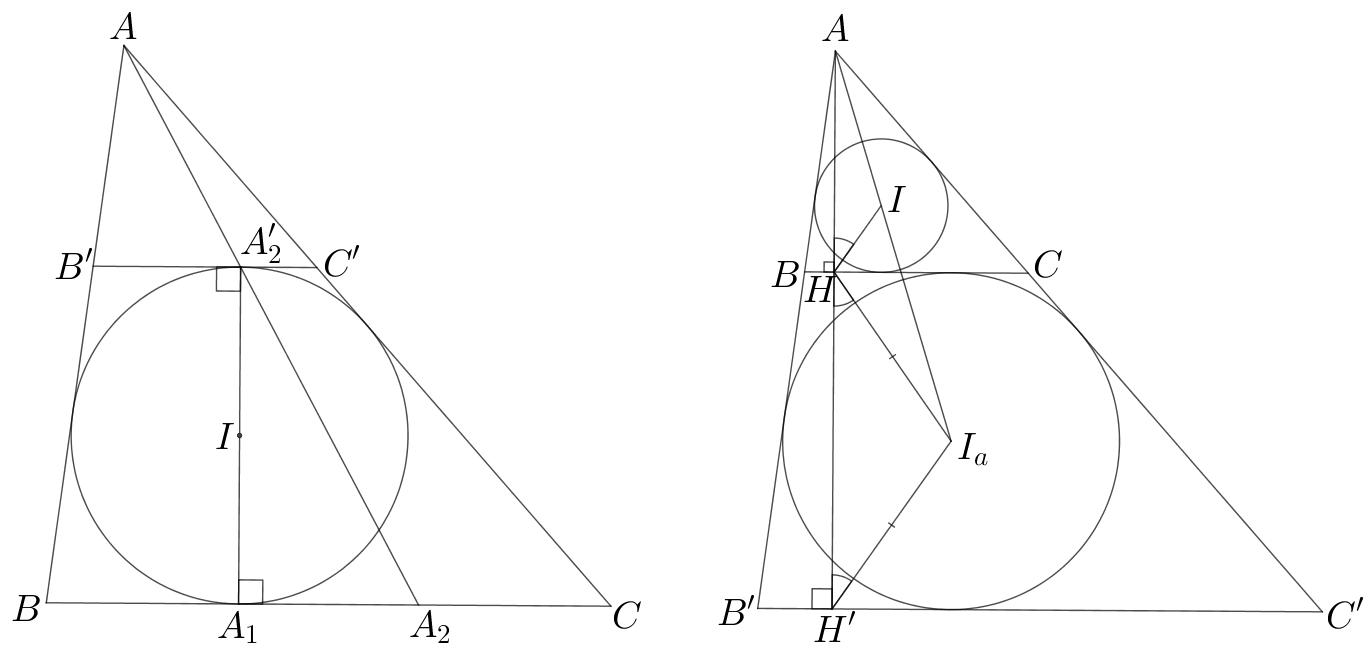
\includegraphics[width=1\textwidth]{Эльзята/G/Homothety/homothety-11.png}
\end{center}

\textbf{Решение (b)} Рассмотрим гомотетию с центром в точке $A$,
которая переводит окружность $\omega$ в окружность $\omega_a$. При этой
гомотетии отрезок $BC$ перейдет в отрезок $B'C'$, касающийся окружности
$\omega_a$ и параллельный $BC$, точка $I$ перейдет в точку $I_a$, а
точка $H$ перейдет в точку $H'$, причем отрезок $AH'$ перпендикулярен
$B'C'$. Поскольку отрезок $HI$ переходит при этой гомотетии в отрезок
$H'I_a$, эти отрезки параллельны, поэтому $\angle AHI=\angle H'HI_a$. С
другой стороны, треугольник $HI_aH'$ является равнобедренным, т.к. точка
$I_a$ равноудалена от параллельных прямых $BC$ и $B'C'$, а отрезок $HH'$
является общим перпендикуляром к этим прямым. Значит,
$\angle H'HI_a=\angle HH'I_a$. Окончательно получаем, что
$\angle AHI=\angle H'HI_a$. Поэтому $\angle IHC=\angle I_aHC$, что и
требовалось доказать.

\begin{center}
    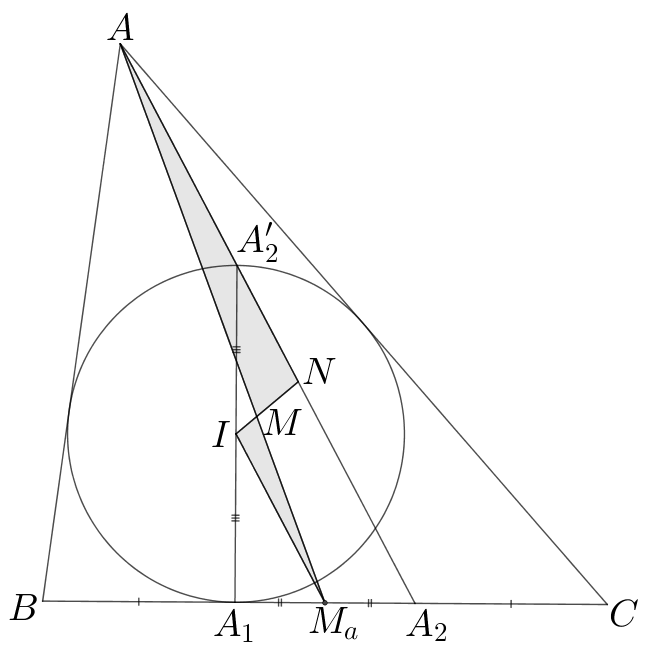
\includegraphics[width=0.5\textwidth]{Эльзята/G/Homothety/homothety-12.png}
\end{center}

\textbf{Решение (c)} Пусть $M_a$ — середина отрезка $BC$. Тогда в силу
равенства отрезков касательных $BA_1=CA_2$, поэтому $M_a$ также является
серединой отрезка $A_1A_2$. Пусть точка $A_2'$ диаметрально
противоположна точке $A_1$ в окружности $\omega$. По задаче <span>**1( a
)**</span> точка $A_2$ лежит на отрезке $AA_2$. Поэтому $M_aI$ — средняя
линия в треугольнике $A_1A_2A_2'$, параллельная прямой $AA_2$.
Рассмотрим гомотетию $H_M^{-2}$. Эта гомотетия переводит точку $M_a$ в
точку $A$, а потому прямая $IM_a$ перейдет в прямую $AA_2$. Значит,
образ точки $I$ при гомотетии $H_M^{-2}$ лежит на прямой $AA_2$.
Аналогично, этот образ должен лежат и на двух других отрезках,
соединяющих вершины $B$ и $C$ треугольника $ABC$ с точками касания
вневписанных окружностей со сторонами $CA$ и $AB$ соответственно.
Получается, что $H_M^{-2}(I)=N$ и точки $I$, $M$ и $N$ лежат на одной
прямой, что и требовалось доказать.

\problem{2}
В треугольник $ABC$ вписана окружность $\omega$. Точки $M_a$, $M_b$ и
$M_c$ — середины сторон $BC$, $CA$ и $AB$ соответственно. Точки $K_a$,
$K_b$ и $K_c$ симметричны точкам касания окружности $\omega$ со
сторонами $BC$, $CA$ и $AB$ относительно биссектрис углов $\angle A$,
$\angle B$ и $\angle C$ соотвественно. Докажите, что прямые $M_aK_a$,
$M_bK_b$ и $M_cK_c$ пересекаются в одной точке.

\textbf{Решение.} Докажем, что стороны треугольников $K_aK_bK_c$ и $M_aM_bM_c$ попарно
параллельны. Обозначим через $G_a$, $G_b$ и $G_c$ точки касания
вписанной окружности $\omega$ со сторонами $BC$, $CA$ и $AB$
соответственно. Тогда четырехугольники $G_aG_cG_bK_b$ и $G_aG_cK_cG_b$
являются трапециями (т.к. их основания перпендикулярны биссектрисам
углов $\angle B$ и $\angle C$ соотвественно), а потому они равнобокие.
Значит, $G_aK_b=G_bG_c=G_aK_c$. Получается, что прямые $K_bK_c$ и $BC$
высекают на окружности $\omega$ равные хорды $G_aK_b$ и $G_aK_c$.
Поэтому эти прямые параллельны. А раз так, что прямая $K_bK_c$
параллельна и средней линии $M_bM_c$ напротив стороны $BC$. Остальные
параллельности проверяются аналогично.

\begin{center}
    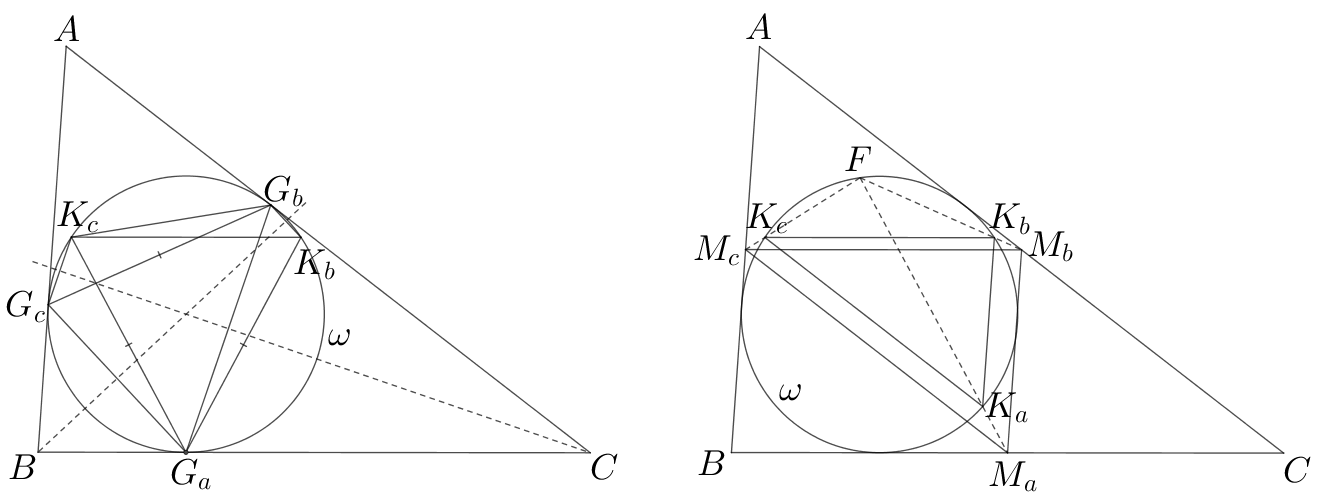
\includegraphics[width=1\textwidth]{Эльзята/G/Homothety/homothety-2.png}
\end{center}

Из теоремы Дезарга следует, что треугольники $K_aK_bK_c$ и $M_aM_bM_c$
гомотетичны. Поэтому прямые $K_aM_a$, $K_bM_b$ и $K_cM_c$ пересекаются в
одной точке $F$ — центре гомотетии этих треугольников, что и требовалось
доказать.

*Замечание*. Можно доказать, что этот центр гомотетии лежит на
окружности $\omega$ и является точкой Фейербаха — точкой касания
вписанной окружности и окружности девяти точек.

\problem{3}
Окружности $\omega_1$, $\omega_2$ и $\omega_3$ попарно касаются друг
друга внешним образом в точках $A$, $B$ и $C$. На окружности $\omega_1$
взята произвольная точка $P$. Прямая $AP$ вторично пересекает окружность
$\omega_2$ в точке $Q$, прямая $QB$ вторично пересекает окружность
$\omega_3$ в точке $R$, а прямая $RC$ вторично пересекает окружность
$\omega_1$ в точке $S$. Докажите, что точки $P$ и $S$ диаметрально
противоположны.

\textbf{Решение.} Обозначим через $H_A$, $H_B$ и $H_c$ гомотетии, которые переводят
соответственно окружность $\omega_1$ в окружность $\omega_2$, окружность
$\omega_2$ в окружность $\omega_3$, окружность $\omega_3$ в окружность
$\omega_1$. Тогда композиция $H_C\circ H_B\circ H_A$ является гомотетией
(т.к. композиция гомотетий есть гомотетия) и переводит окружность
$\omega_1$ в себя. Заметим, что т.к. у всех гомотетий $H_A$, $H_B$ и
$H_C$ отрицательные коэффициенты, коэффициент их композиции, равный
произведению коэффициентов отдельных гомотетий, также отрицателен.
Поэтому данная композиция гомотетий является центральной симметрией.
Т.к. эта симметрия сохраняет окружность $\omega_1$, ее центр совпадает с
центром окружности $\omega_1$. Поэтому образ $S$ точки $P$ при этой
композиции будет диаметрально противоположен $P$, что и требовалось.

\begin{center}
    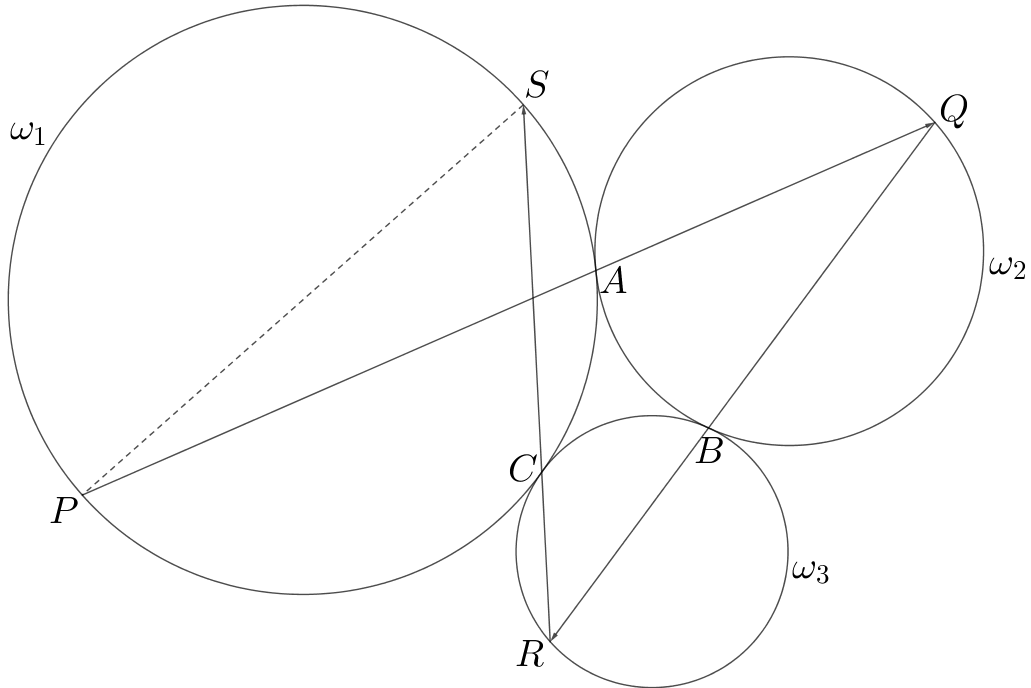
\includegraphics[width=0.6\textwidth]{Эльзята/G/Homothety/homothety-3.png}
\end{center}

\problem{4}
В треугольнике $ABC$ проведена биссектриса $AD$. Общая касательная
$\ell$ к окружностям $(ABD)$ и $(ACD)$ касается их в точках $M$ и $N$
соответственно. Докажите, что прямая $\ell$ касается окружности,
проходящей через середины отрезков $MN$, $BD$, $CD$.

\textbf{Решение.} Рассмотрим точку $O$ пересечения прямых $BC$ и $\ell$ и рассмотрим
гомотетию $H_O^k$ с центром в $O$, которая переводит окружность $(ABD)$
в окружность $(ACD)$. Ясно, что коэффициент $k$ равен отношению радиусов
окружностей $(ABD)$ и $(ACD)$, а также $H_O^k(B)=D$. Заметим, что по
теореме синусов $BD:CD=k$, поэтому $H_O^k(D)=C$. Значит, гомотетия
$H_O^k$ переводит треугольник $MBD$ в треугольник $NDC$. Но тогда
гомотетия $H_O^{k/2}$ переводит треугольник $MBD$ в треугольник с
вершинами в серединах отрезков $MN$, $BD$ и $CD$. Поэтому окружность
$H_O^{k/2}((MBD))$ проходит через эти середины и касается прямой $\ell$,
что и требовалось доказать.

\begin{center}
    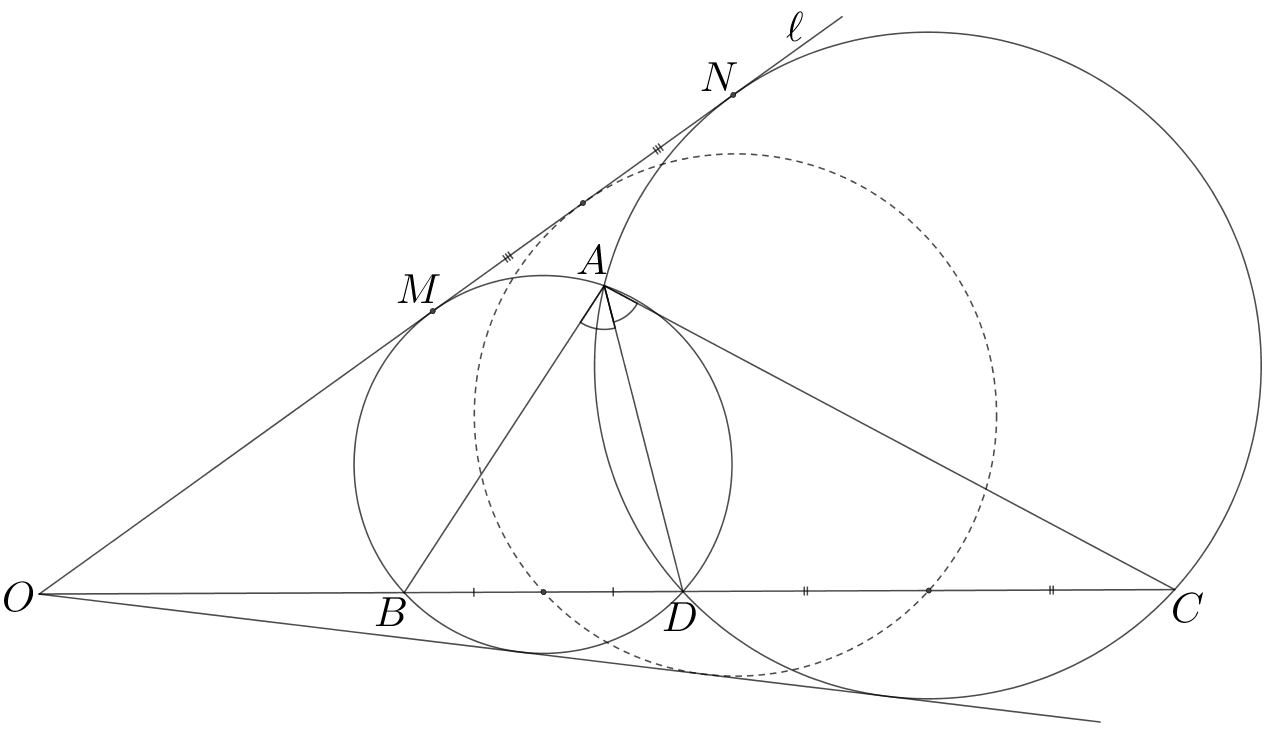
\includegraphics[width=0.9\textwidth]{Эльзята/G/Homothety/homothety-4.png}
\end{center}

\problem{5}
В остроугольном треугольнике $ABC$ проведена высота $AA_1$ и отмечена
точка $M$ пересечения медиан. Луч $MA_1$ пересекает окружность $(ABC)$ в
точке $K$. Докажите, что окружность $(A_1BK)$ касается прямой $AB$.

\textbf{Решение.} Рассмотрим гомотетию $H_M^{-2}$. Эта гомотетия переведет треугольник
$ABC$ в треугольник $A_0B_0C_0$, для которого точки $A$, $B$ и $C$ будут
серединами сторон, а окружность $(ABC)$ будет окружностью Эйлера.
Значит, образ $A'$ точки $A_1$ при этой гомотетии будет лежать на
окружности $(ABC)$, т.к. точка $A_1$ будет основанием высоты в
треугольнике $A_0B_0C_0$, проведенной из вершины $A$. Получается, что
четырехугольник $AA'CB$ является вписанной трапецией, а потому углы при
ее основании $BC$ равны. Значит, $\angle A_1KB=\angle A'CB=\angle ABC$,
и прямая $AB$ касается окружности $(A_1BK)$ по обратной теореме об угле
между касательной и хордой.

\begin{center}
    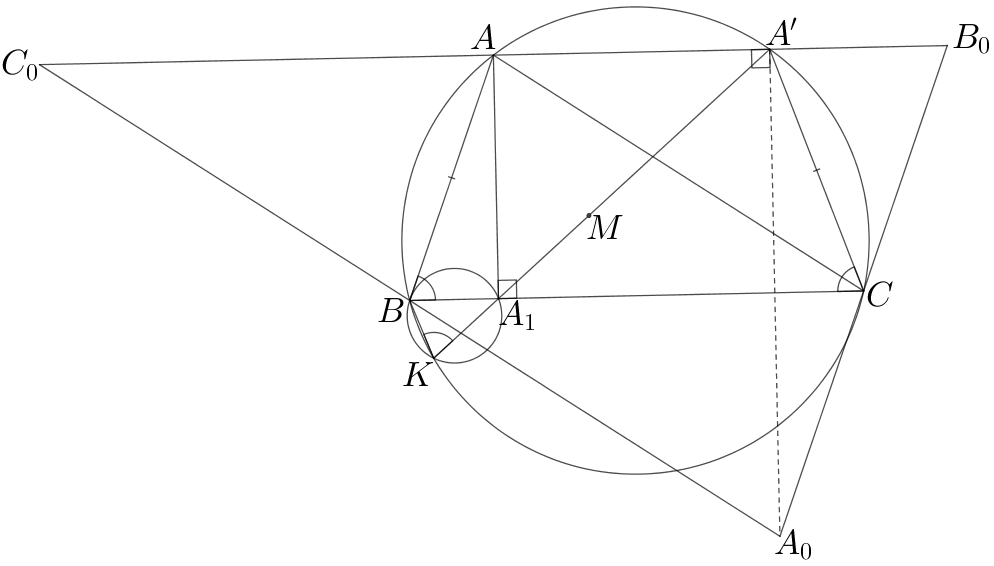
\includegraphics[width=0.8\textwidth]{Эльзята/G/Homothety/homothety-5.png}
\end{center}

\problem{6}
В треугольник $ABC$ вписана окружность $\omega$ с центром в точке $I$,
касающаяся стороны $BC$ в точке $D$. Пусть $\omega_B$ и $\omega_C$ —
вписанные окружности треугольников $ABD$ и $ACD$ соответственно,
касающиеся стороны $BC$ в точках $E$ и $F$ соответственно. Пусть $P$ —
точка пересечения отрезка $AD$ с линией центров окружностей $\omega_B$ и
$\omega_C$, $X$ — точка пересечения прямых $BI$ и $CP$, $Y$ — точка
пересечения прямых $CI$ и $BP$. Докажите, что прямые $EX$ и $FY$
пересекаются на окружности $\omega$.

\textbf{Решение.} Прежде всего заметим, что окружности $\omega_B$ и $\omega_C$ касаются
друг друга и отрезка $AD$ (это следует из счета отрезков касательных).
Поэтому они касаются друг друга в точке $P$.

Пусть $D'$ — точка, диаметрально противоположная точке $D$ в окружности
$\omega$. Докажем, что точка $D'$ лежит на прямой $EX$ (для прямой $FY$
рассуждения аналогичны). Для этого рассмотрим точку $X'$ пересечения
прямых $ED'$ и $CP$ и докажем, что $X'=X$. В самом деле, точка $P$ —
центр гомотетии с отрицательным коэффициентом для окружностей $\omega_B$
и $\omega_C$, точка $C$ — центр гомотетии с положительным коэффициентом
для окружностей $\omega_C$ и $\omega$, а точка $X'$ — центр гомотетии с
отрицательным коэффициентом для окружностей $\omega_B$ и $\omega$. По
теореме о трех центрах гомотетий эти три точки лежат на одной прямой, а
значит, $X'=X$, что и требовалось.

\begin{center}
    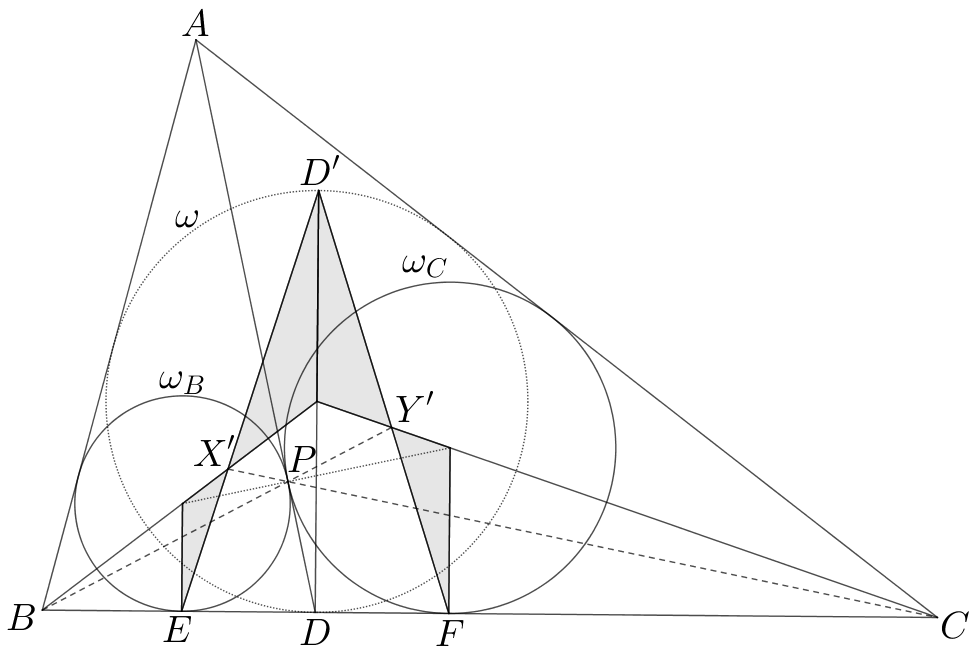
\includegraphics[width=1\textwidth]{Эльзята/G/Homothety/homothety-6.png}
\end{center}



\problem{7}
Две окружности $\Omega$ и $\omega$ касаются в точке $A$. Прямая $\ell$
пересекает окружность $\Omega$ в точках $B$ и $C$ и касается окружности
$\omega$ в точке $D$. Докажите, что прямая $AD$ проходит через середину
дуги окружности $\Omega$, стягиваемую хордой $BC$ (разберите случаи
внешнего и внутреннего касания).\

Рассмотрим гомотетию $H_A$, переводящую окружность $\omega$ в окружность
$\Omega$. Тогда точка $D$ перейдет в точку $D'$ на окружности $\Omega$,
а касательная $\ell$ к окружности $\omega$ перейдет в касательную
$\ell'$ к окружности $\Omega$. Прямые $\ell$ и $\ell'$ параллельны,
поэтому они высекают на окружности $\Omega$ равные дуги. Значит, точка
$D'$ является серединой дуги $BC$ окружности $\Omega$, что и требовалось
доказать.

\begin{center}
    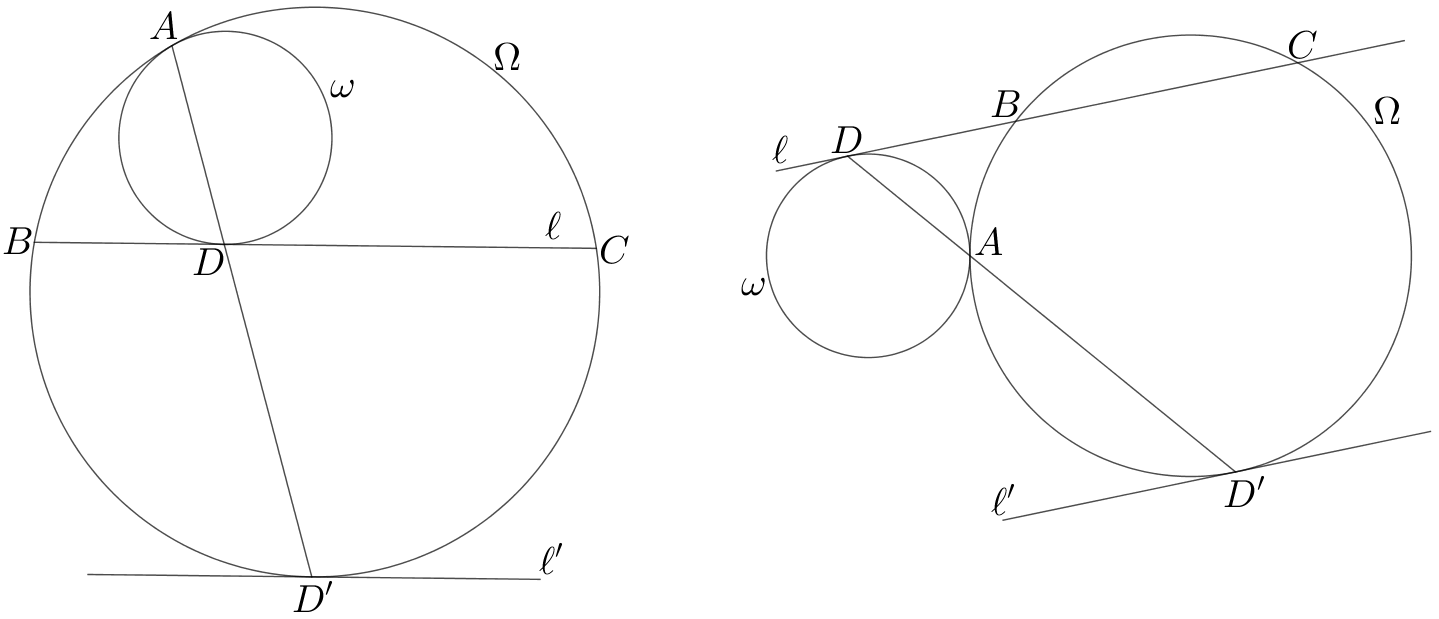
\includegraphics[width=1\textwidth]{Эльзята/G/Homothety/homothety-71.png}
\end{center}

\problem{8}
Вокруг равнобедренного треугольника $ABC$ ($AB=AC$) описана окружность
$\Omega$. Окружность $\omega$ касается сторон $AB$ и $AC$ в точках $K$ и
$L$ и касается внутренним образом окружности $\Omega$. 

(a) Докажите, что центр вписанной окружности треугольника $ABC$ лежит на отрезке $KL$.\

(b) Докажите утверждение предыдущего пункта для произвольного треугольника
$ABC$.

\textbf{Решеение (b)} Пусть $T$ — точка касания окружностей $\Omega$ и
$\omega$. Проведем прямую $TL$, и пусть она вторично пересекает
окружность $\Omega$ в точке $W$. По лемме Архимеда точка $W$ — середина
дуги $AC$ окружности $\Omega$, поэтому прямая $BW$ является биссектрисой
угла $\angle B$, а точка $I$ пересечения прямых $AT$ и $BW$ — центром
вписанной окружности треугольника $ABC$. Поэтому $CI$ — биссектриса угла
$\angle C$, откуда следует цепочка равенств
$\angle ACI=\angle BCI=\angle CBI=\angle CTW=\angle LTI$. Значит,
четырехугольник $CTIL$ является вписанным. Заметим, что угол
$\angle ACT$ прямой, т.к. смотрит на диаметр $AT$ окружности $\Omega$,
поэтому $\angle AIL=\angle ACT=90^\circ$. Получается, что $IL$
перпендикулярно $AT$. Аналогично $IK$ перпендикулярно $AT$. Значит,
точки $K$, $I$ и $L$ лежат на одной прямой, что и требовалось доказать.

\begin{center}
    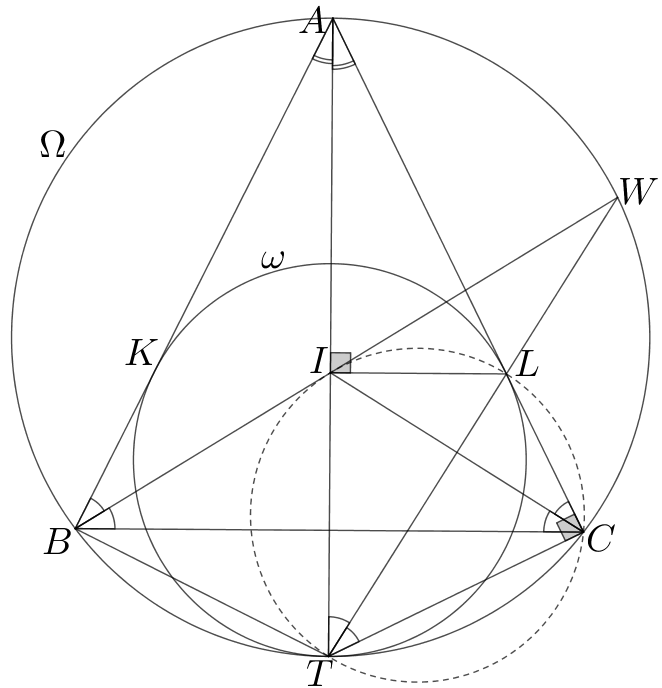
\includegraphics[width=0.8\textwidth]{Эльзята/G/Homothety/homothety-72.png}
\end{center}

\textbf{Решение (c)} Пусть $T$ — точка касания окружностей $\Omega$ и
$\omega$. Проведем прямые $TK$ и $TL$, и пусть они вторично пересекают
окружность $\Omega$ в точках $W_b$ и $W_c$ соответственно. По лемме
Архимеда точки $W_b$ и $W_c$ — середины дуг $AC$ и $BC$ окружности
$\Omega$, поэтому прямые $BW_b$ и $CW_c$ являются биссектрисами углов
$\angle B$ и $\angle C$ соответственно, а точка $I$ их пересечения
является центром вписанной окружности треугольника $ABC$. Применим
теорему Паскаля к шестивершиннику $BACW_cTW_b$ и получим, что точки $K$,
$I$ и $L$ лежат на одной прямой, что и требовалось доказать.

Сначала заметим, что треугольники $WCT$ и $WLC$ также подобны по двум
углам: угло при вершине $W$ у них общий, а также
$\angle WTC=\angle WBC=\angle ABW=\angle WCL$. Значит, эти треугольники
подобны по двум углам, откуда $WL:WC=WC:WT$ и $WC^2=WL\cdot WT$.

\begin{center}
    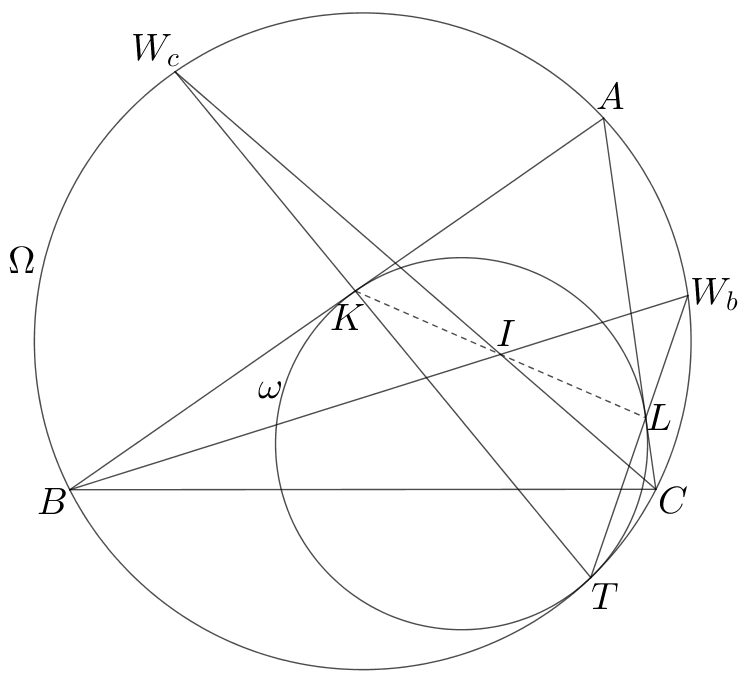
\includegraphics[width=0.5\textwidth]{Эльзята/G/Homothety/homothety-73.png}
\end{center}

Теперь будем доказывать подобие треугольников $WIT$ и $WLI$. Начнем с
того, что отметим точку $Q$ пересечения биссектрисы $BW$ и отрезка $AC$.
Точки $B$, $T$, $L$ и $Q$ лежат на одной окружности:
$\angle CBQ=\angle ABQ=\angle ACW$ и $\angle CBT=\angle CWT$, откуда
$$\angle TBQ=\angle TBC+\angle CBW=\angle CWLL+\angle LCW=\angle CLT$$
(последнее равенство есть теорема о внешнем угле в треугольнике $CLW$).
Теперь заметим, что на одной окружности лежат точки $B$, $I$, $K$ и $T$.
В самом деле, $\angle TBI=\angle TLC=\angle TKL$. наконец, докажем
подобие треугольников $WIT$ и $WLI$. Угол при вершине $W$ у них общий, а
также $\angle BIT=\angle BKT=\angle ILT$, откуда
$\angle WIT=\angle WLI$. Значит, эти треугольники подобны по двум углам,
откуда $WL:WI=WI:WT$ и $WI^2=WL\cdot WT$.

Таким образом, $WC^2=WL\cdot WT=WI^2$ и $WC=WI$. Поэтому из теоремы о
трезубце следует, что точка $I$ является центром вписанной окружности
треугольника $ABC$, что и требовалось доказать.
